\section{Running Example: Sensor System}
\label{sec:sensorExample}
We present a running example of a simplified sensor system in a Pressurized Water Reactor (PWR). In a typical PWR, the core inside of the reactor vessel produces heat. Pressurized water in the primary coolant loop carries the heat to the steam generator. Within the steam generator, heat from the primary coolant loop vaporizes the water in a secondary loop, producing steam. The steamline directs the steam to the main turbine, causing it to turn the turbine generator, which produces electricity. There are a few important factors that must be considered during safety assessment and system design. An unsafe climb in temperature can cause high pressure and hence pipe rupture, and high levels of radiation could indicate a leak of primary coolant~\cite{PWR}. 

\begin{figure*}[h!]
	%\vspace{-2em}
	\begin{center}
		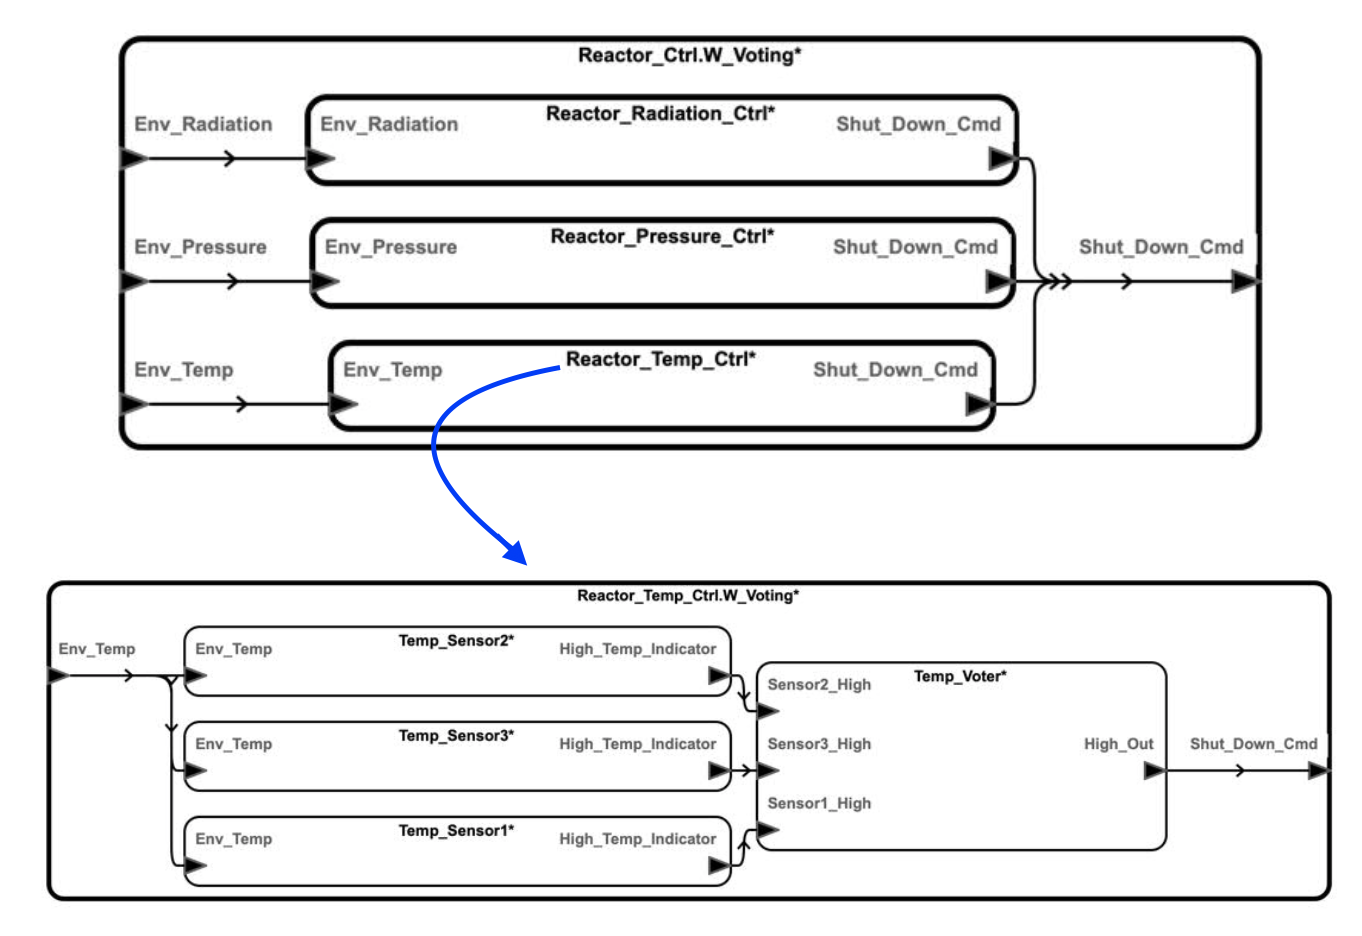
\includegraphics[width=0.6\textwidth]{images/sensorSysAADL.png}
	\end{center}
	\vspace{-2em}
	\caption{PWR Sensor System}
	\label{fig:sensorSys1}
	%\vspace{-2em}
\end{figure*}

The following sensor system can be thought of as a subsystem within a PWR that monitors these factors. A diagram of the model is shown in Figure~\ref{fig:sensorSys1} and represents a highly simplified version of a safety critical system. The temperature subsystem details are shown at the bottom of Figure~\ref{fig:sensorSys1}; each of the subsystems have a similar architecture.

The subsystems each contain three sensors that monitor pressure, temperature, and radiation. Environmental inputs are fed into each sensor in the model and the redundant sensors monitor temperature, pressure, or radiation respectively. If temperature, pressure, or radiation is too high, a shut down command is sent from the sensors to the parent components. 

\subsubsection{PWR Nominal Model}
The temperature, pressure, and radiation sensor subsystems use a majority voting mechanism on the sensor values and will send a shut down command based on this output. The safety property of interest in this system is: \emph{shut down when and only when temperature, pressure, or radiation is above the respective threshold}; the AGREE guarantee stating this property is shown in Figure~\ref{fig:shutdownGuar}. 

\begin{figure*}[h!]
	%\vspace{-2em}
	\begin{center}
		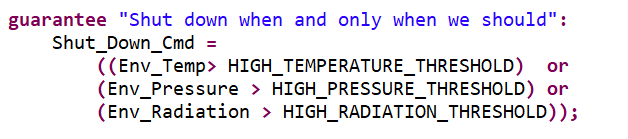
\includegraphics[width=0.6\textwidth]{images/sensorGuar.PNG}
	\end{center}
	\vspace{-2em}
	\caption{Sensor System Safety Property}
	\label{fig:shutdownGuar}
	%\vspace{-2em}
\end{figure*}

The safety of the system requires a shut down to take place if the temperature, pressure, or radiation levels climb beyond safe levels; thus, a threshold for each subsystem is introduced. If any sensor subsystem reports passing its threshold, a shutdown command is sent. Supporting guarantees are located in each sensor subsystem and correspond to temperature, pressure, and radiation sending a shut down command if sensed inputs are above a given threshold. Each sensor has a similar guarantee. 

Throughout the remainder of this chapter, we refer to the PWR example for illustrative purposes. The goal is to take the nominal system model and extend it to become a fault model using the safety annex. 